\begin{abstract}
This paper describes the development of an industrial safety system that requires automatic human detection. Two solutions based on top-view depth images are presented. The first one is based on traditional learning techniques using feature extraction and a Support Vector Machine classifier. The second solution uses deep learning methods for classification. The performance analysis of both solutions revealed that the deep learning methods outperform traditional learning techniques on this task, at the cost of requiring a larger training set and increased computational cost.
\keywords{Human Detection \and Depth Images \and Deep learning \and Convolutional Neural Networks}
\end{abstract}

\section{Introduction}
  In any industrial facility workers safety must be a priority. There are certain areas that offer higher risk and thus should not be occupied during regular operation. An example is given by a home appliance factory that uses an overhead crane to shift iron molds towards plastic extruding machines. These molds can be very heavy, offering risks to anyone working underneath the moving crane.

  In this context it is helpful to have an automatic safety system that detects humans on the path of the moving machine and causes it to halt in the event it finds a person. A video based solution would be ideal in this case, especially considering that the factory environment is crowded with machines, molds and workers. Since the crane will be moving, the camera should be placed underneath it, facing the factory floor. The non-static background poses a challenge as common background subtraction methods cannot be applied, requiring a more sophisticated detection algorithm.

  Another challenge is that workers clothes are not regular in color, and they do not always wear helmets, in which case only color images could not give enough information for detection. To overcome this, \cite{rauter} uses a stereo camera that delivers depth image frames of objects, providing more reliable shape information and higher invariance to luminosity. The image is then used to locate human candidates, followed by a hand-engineered feature extraction and then classification using a Support Vector Machine (SVM). However, it assumes a clean standard ambient, where there are only people and in some cases luggage moving around, and thus may not provide a good solution to a complex and crowded industrial environment, with many machines and equipment among workers.

  Recently the increase of computational power, especially in the form of GPUs, the availability of large image datasets and improvements upon existing training methods \cite{nair2010relu} enabled the fast development and usage of deep learning methods in most diverse domains. Moreover, novel dense network structures \cite{NIPS2013_5207} achieved great results for object detection, following previous state-of-the-art results \cite{hintonCONVNET} for image classification. The main advantage of deep learning methods is that they shift the focus from feature-engineering to a data-driven approach. In this sense the network structure itself will learn how to best represent the input data, as long as it has enough samples to learn from. Although some object classification with deep-based classifiers, such as \cite{thornberg2015combining}, use depth images they do not assume a overhead position of the camera. To the best of our knowledge, a deep classifier solution for top-view human detection using depth frames has not been proposed so far.

  This paper presents a novel top-view human detection system based on deep classifiers. We also perform a comparison between the proposed method and a traditional approach to the human detection system, illustrated in Figure \ref{fig:system-diagram}. Both use computer vision techniques to detect candidates in the image, described in Section \ref{sec:candidates}. The traditional solution, based in \cite{rauter}, is presented in Section \ref{sec:classical}, while our solution, using deep classifiers, is described in Section \ref{sec:deep}. Quantitative evaluation of both methods and their variations is shown in Section \ref{sec:results}. Finally, conclusions and future work are presented in Section \ref{sec:conclusion}.

  \begin{figure*}[!t]
  \centering
  \includegraphics[width=\linewidth]{system-diagram.png}
  \caption{Human detection system diagram. Two candidates are detected on the input frame.  }
  \label{fig:system-diagram}
  \end{figure*}

\section{Candidates detection}
\label{sec:candidates}

    In a traditional object detection approach \cite{traditional-objdetect} the first step is to localize candidates, which are then validated using a feature-extractor followed by a classifier. In the case of a color image, a sliding window method with varying size could be used to obtain such candidates.

    However, when using depth images from a top-view scene, \cite{rauter} suggests a more efficient algorithm that assumes that humans will be among the highest objects in the scene. Although this hypothesis cannot always be guaranteed, it reduces the amount of candidates significantly when compared to the sliding window method and so is used in this work and described next.

    First, a local maxima operation is performed. It divides the image in a grid of specified-sized blocks and for each block returns the pixel with highest intensity, representing the tallest point in that block. Next, for each local maxima a squared window representing the candidate should be obtained. Its size is calculated as
    \begin{equation}
      s_w = \frac{f}{d} \cdot s_r
    \end{equation}
    where $f$ is the camera focal distance, $d$ the distance between the camera and the object and $s_r$ the mean head size. The window of size $s_w$ pixels is centered around the respective local maximum pixel.

    The final step is to centralize the window over the candidate using an iterative \textit{mean shift} algorithm. Simply put, this algorithm displaces the window to the centroid of the pixels inside it, so high valued pixels will tend to be in the center of the candidate.

    The output of this step is a list of squared windows representing candidates in the image. A relevant aspect to consider is the size of the blocks for the local maxima search. When using large blocks the probability of having a tall object, such as a machine, in the same block of a person is high, so the system would fail to detect a person. In contrast, if the block is too small, it is guaranteed that all humans will be detected, but this comes at the expense of complexity and time performance, since all candidates will need further analysis.

\section{Classical computer vision solution}
\label{sec:classical}

    Following the candidates detection a validation phase should take place to discard non-human detections. A classical computer vision approach \cite{rauter} uses hand-engineered features extracted from the candidates to feed a binary SVM classifier, which output a class: ``human'' or ``not human''. A regular block grid proposed in \cite{rauter} is used. In order to increase rotation invariance, we also propose a concentric rings descriptor (see Figure \ref{fig:descriptors}). Both are described next, followed by a more detailed description of the classification and training process.

    \begin{figure}
    \centering
    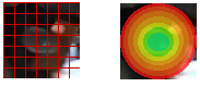
\includegraphics[width=0.9\linewidth]{tradicional/descritores}
    \caption{Regular block grid (left) and concentric rings descriptors (right).}
    \label{fig:descriptors}
    \end{figure}

    \subsection{Regular block grid feature extractor}
      This descriptor divides the candidate window into 7x7 blocks, as illustrated in Figure \ref{fig:descriptors}. The mean value of pixels belonging to each block is calculated, generating a 7x7 matrix of mean pixel intensities. Next, the mean value of the central block is subtracted from the matrix. Finally, the resulting matrix histogram is calculated with 32 bins. The histogram vector, with 32 dimensions, is considered the feature vector, which sums up to 49 (number of blocks).

    \subsection{Concentric rings feature extractor}
       First the candidate window is divided in 18 annulus, or rings, with equal distance between the inner and outer radius and whose center coincides with the window center. Then for each ring the mean of the pixels that belong to it is calculated, resulting in a 18 dimensional vector of mean pixel intensity. Next, the mean value of the inner ring (lower radius equals zero) is subtracted from this vector. Following, we perform a discrete differentiation of this vector (subtraction between adjacent dimensions) to enunciate the differences in rings mean values, resulting in a 17-dimensional feature vector.

    \subsection{SVM classifier}
      We use a binary SVM classifier with Radial Basis Function (RBF) kernel \cite{rbfkernel} to validate the candidates. Recall that the kernel parameter $\sigma$ along with the SVM hyperparameter $C$ control the trade-off between training performance and generalization on unseen data. Higher $C$ values penalize training set errors, while lower values offer a more general performance on the test set, conversely, the $\sigma$ parameter penalizes in the inverse manner.

      To choose the appropriate values of the hyperparameters $C$ and $\sigma$ we use a 5 fold cross-validation process, scoring the \textit{recall} metric \cite{evaluationMetrics}. After the hyperparameters have been chosen the final training process is carried out with the entire training dataset using the Scikit-learn \cite{scikit-learn} toolkit. The training time takes 1 minute and 36 seconds for the regular block grid descriptor and 25s for the ring grid descriptor on an Intel i7 CPU.


\section{Deep learning based solution}
\label{sec:deep}

    Neural networks can be used to perform robust classification with complexity varying according to the network structure and depth. A regular artificial neural network is composed by units organized in layers with every unit in a single layer connected to every unit on the following layer. Each unit calculates its output by summing its inputs, weighted by the connections parameters, and then applying an activation function $\phi(x)$. The output is forward propagated through the network from the input layers, through the hidden layers until the output layer.

    In images there is strong local correlation of pixels, so it is not necessary that every unit in each layer is connected to every unit in the following layer, but just to a few local neighbors. This local connectivity is achieved through the convolution of a given layer with a bank of filters. In this sense, convolutional neural networks give a better model for images by reducing the number of parameters thus helping generalization.

    We propose a convolutional network based classifier that receives the candidate image without any feature-extraction process. The model itself will encode a feature map as the convolutional layers are applied, with the final layer doing the classification process and outputting a single probability of that candidate being a human. This system diagram would be the same as presented in Figure \ref{fig:system-diagram} without the feature extraction block and with a real valued output probability.

    \subsection{Network architecture}
        The first layer used is a batch normalization layer \cite{DBLP:journals/corr/IoffeS15} that normalizes the input batch to zero mean and unit variance, then scales and shift it using additional parameters learned during training. Although this technique is rather explored to avoid the covariance shift in internal layers, it has been proved an eficient method to speed up network convergence \cite{DBLP:journals/corr/IoffeS15}. Additionally, we found that this layer positively impacted the optimization convergence, which had significantly bad performance as the training set is highly unbalanced, as described in Section \ref{sec:dataset}. Since candidates can have arbitrary size, the first step is to resize them to a fixed 60 x 60 window. This guarantees a fixed size input to the network.

        Following the Visual Geometry Group approach on the ImageNet challenge \cite{Simonyan14c}, an architecture of stacked small filters convolutional and max pooling layers is used. This choice is particularly interesting because it can cover the same receptive field in the input image as a single conv layer with a bigger filter, but with less parameters. Additionally, it has been shown \cite{Simonyan14c} to increase classification performance when compared to the latter method. The convolution operation is done with 3 x 3 filters and uses input padding to keep the output dimensions constant. Dimensionality reduction is achieved across the network by 2 x 2 max pooling layers after each convolutional layer.

        After the convolutional stage we obtain a feature map which is then flattened and introduced to a dense layer with a single output unit. All the network uses the RELU \cite{nair2010relu} activation function to avoid the vanishing gradient problem common in deep nets. An exception is made for the output unit, which uses the sigmoid function since it should be interpreted as a probability.

    \subsection{Hyperparameter search}
        A natural question that arises when designing the architecture is the number of convolutional layers it should have. Having a small amount of convolutional layers will result in a high dimensional feature map, thus shifting most of the network parameters to the classification dense layer. In contrast, an excessive deep network may be too slow for real time operation. The number of convolutional layers can range up to 5, as the feature map size decreases in half after each layer.

        To choose this hyperparameter we ran training experiments with networks ranging from 1 to 5 conv layers for 50 epochs. We also adjusted the number of filters of each network so that the amount of parameters would be mostly the same, at around 1800, so a fair comparison could be made. The initial parameters of the network have a big impact on the final performance, as the initialization of some parameters may lead to local minima. To reduce the impact of the initial values of parameters, we ran 40 training trials for for each choice of the number of layers, evaluating the Matthews correlation coefficient \cite{evaluationMetrics} on the validation set (30\% split on training set). The best run of each choice of layer count was selected. The results presented in Table \ref{table:evalNumberConvLayers} show that the performance improves as more convolutional layers are added. Although the increase in performance is not drastical we decided to use a 5 convolutional layer network, especially considering that the time penalty for using such an architecture is not too high. Note that although

      	\begin{table}
      	 \begin{center}
      	  \label{table:evalNumberConvLayers}
      	  \caption{Evaluation of networks with different number of convolutional layers. Columns indicate the total amount of parameters of the network, the dimension of the feature map (flattened output of last convolutional layer), Matthews score on validation set and evaluation time (on validation set with 929 samples), respetively.}
      	  \begin{tabular}{ | l | c | l | c | c |}
      	    \hline
      	    \#Conv layer & \#Params & Feature map dim & Score & Eval time (ms)   \\ \hline
      	    1            & 1825    &  1800           & 0.865 &  596             \\
      	    2            & 1745    &  1350           & 0.884 &  968             \\
      	    3            & 1645    &  392            & 0.883 &  1050            \\
      	    4            & 1909    &  72             & 0.887 &  1080            \\
      	    5            & 1874    &  7              & 0.891 &  1260            \\ \hline
      		  \end{tabular}
      		\end{center}
      	 \end{table}

        The number of filters per convolutional layer is another hyperparameter that must be choosen carefuly to adjust the model capacity. By increasing the number of filters the network will be able to handle more complex image structures, but may overfit if there is not enough data. There is also an increase in the computation time when adding more filters. So, clearly the number of filters per layer must be chosen carefully. Having established the number of convolutional layers, we ran a following series of training experiments using 50 epochs for training, 30\% validation split, and getting the best result for 20 training trials to reduce the effect of weights initialization and local minima. The results are reported on Table \ref{table:evalNumberFilters}.

        \begin{table}
      	 \begin{center}
      	  \label{table:evalNumberFilters}
      	  \caption{Evaluation of 5-layer networks with varying number of convolutional filter. Columns indicate number of convolutional filters per layer, total amount of parameters of the network, Matthews score on validation set and evaluation time (on validation set with 929 samples), respectively.}
      	  \begin{tabular}{ | l | c | c | c |}
      	    \hline
      	    \#Filters  & \#Params  &  Score   & Eval time (ms)   \\ \hline
      	    4,4,8,8,16 &   2257    &  0.8584  &    824           \\
      	    8,8,8,8,8  &   2429    &  0.8614  &    1110           \\ \hline
      		  \end{tabular}
      		\end{center}
      	 \end{table}

        The results suggest that having more filters per layer provide a better result without significantly enlarging the evaluation time. So we defined our architecture to be a 5-layer convolutional network with 8 filters per convolutional layer, yielding a 2429 parameters model.


    \subsection{Training}
        The training process consists of minimizing an objective function, in this case, the binary cross-entropy function \cite{DLbook}, also known as log-loss. Its use is justified by the probabilistic nature of the output layer. The optimization method used is a variation of Batch Stochastic Gradient Descent (B-SGD) called Adagrad \cite{duchi2011adaptive}, which uses an adaptive learning rate for each parameter based on the frequency it is updated.

        The ideal number of epochs used for training was found through a validation curve, generated using a 70\% split of the trainng set, evaluated using the Matthews metric, observed in Figure \ref{fig:validation_curve}. It is possible to see a saturation of the validation performance between 20 and 30 epochs and a slow tendency to overfit after 40 epochs. The ideal number of epochs was then chosen to be 30. Note that the training will use the whole training set, not the 70\% split used in this evaluation.

        \begin{figure}
        \centering
        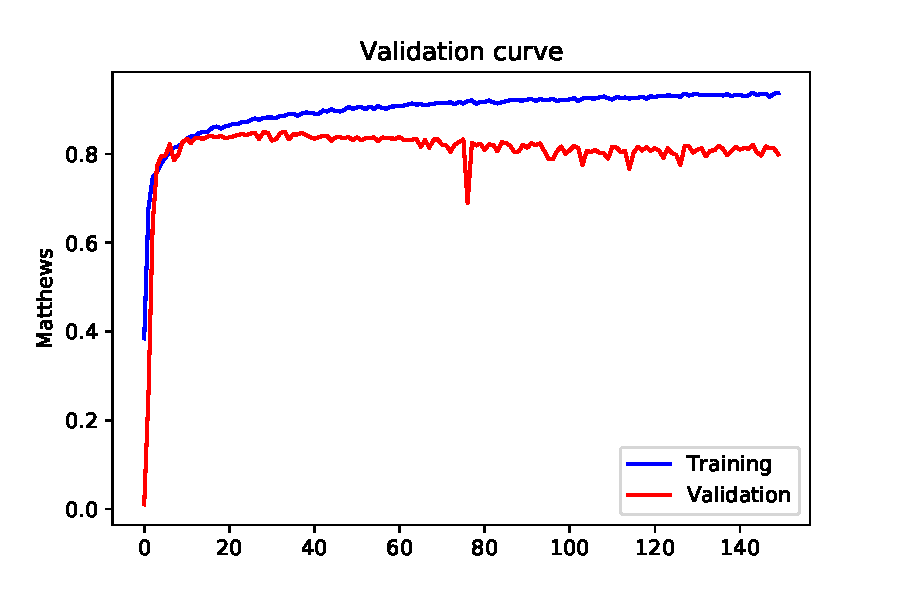
\includegraphics[width=\linewidth]{results/validation_curve.pdf}
        \caption{Validation curve up to 150 epochs. 70\% split on training set.}
        \label{fig:validation_curve}
        \end{figure}

        We experimented two regularization techniques. Primarily we used L2 regularization on the convolutional kernels in two scales, with $\lambda = 0.01$ and $\lambda = 0.1$. In the first case the model performance was similar to the model obtained without regularization. In the second case, the model was prevented to learn the data underlying structure due to the strong regularization applied, causing underfitting. Another technique used was adding a Dropout layer after every convolutional layer. The drop rate used was 20\% and the results consistently shown that regularization degraded the model performance. In conclusion, since the results using regularization techniques were not satisfactory when compared to the standard approach, and considering the validation curve on Figure \ref{fig:validation_curve}, which indicates that no overfit occurs before 30 epochs, we decided to train the model without regularization techniques.

        We observe that the dataset is extremely unbalanced, having more than seven times the amount of negative rather than positive samples, as described in Section \ref{sec:dataset}. To artificially balance the samples, data augmentation was performed by using random rotation and shifts in the positive samples until their number was approximately the same as the negative ones. We evaluated training using this balanced dataset but there was no significant improvement on the validation set performance. Due to new transforme samples the training time increased so we decided to keep the original training set without augmentation.

	The final model was learned with the original, unbalanced, training set for 30 epochs and without regularization. The time required for training was 5 minutes and 31 seconds on CPU and 50.3 seconds on a NVIDIA GTX 1060 GPU.

        Regarding implementation, the computer vision tasks (candidate extraction, resizing) were done using the OpenCV library. The deep classifier was implemented using Keras \cite{keras} with the TensorFlow \cite{tensorflow2015-whitepaper} backend.

\section{Dataset}
\label{sec:dataset}
The dataset was generated through video sequences recorded with the StereoLabs ZED depth camera during a one time visit to the factory. All these videos were recorded with the camera fixed at the bottom of the crane at a height of 6m during the morning with constant and standard indoor illumination. Each video shows distinct workers on their tasks with the crane occasionally moving along the plant, and although some machines and objects are seen repeatedly, no single individual appear on distinct videos. Two video samples are selected exclusively for training and the two remaining for the test set.

The training set was generated by selecting the reserved video samples and applying the candidate detection algorithm, as shown in Figure \ref{fig:dataset}, manually labelling each candidate as a person or not. Each sample in this set is the corresponding candidate slice of the depth image (the region delimted by the bounding boxes in the second column of Figure \ref{fig:dataset}). This allowed us to get 14966 negative and 1932 positive samples in this set. It is important to note the highly biased nature of the training set: more than 88\% of the samples belong to the negative class.

There are two types of test sets: the candidate and whole frames test set. The first one is used to evaluate the classifiers individually, while the latter can be used to assess the whole system performance. To generate the candidate test set the same process used for training set generation is repeated, but using the reserved test video sequences, obtaining 2738 negative and 235 positive samples. The whole-frames test set is generated by selecting a number of frames from the reserved videos and labelling them as positive (at least one person appears) or not. This results in a set composed by 2334 positive and 66 negative frames.

This dataset poses a few challenges, such as seen in Figure \ref{fig:dataset} (c): a worker on the top left side is not detected because he is occluded by the crane carrying a mold. Another issue is when candidates resemble a head in its shape, such as the bucket on the middle right of Figure \ref{fig:dataset} (e).  For privacy reasons the company who owns the factory did not allow the video sequences to be made publicly available.

\begin{figure*}[!t]
\centering
\subfloat[]{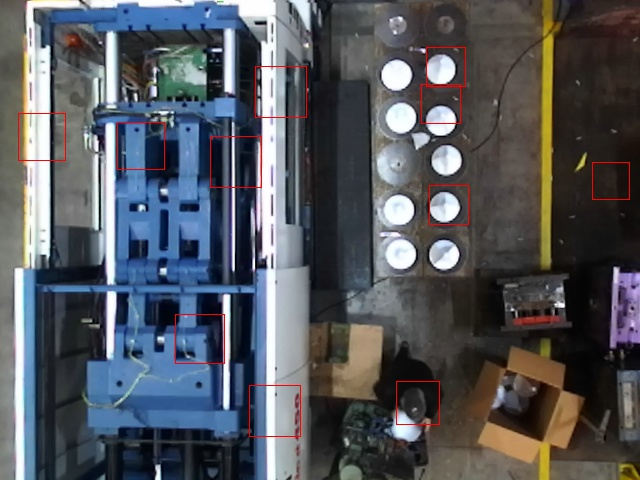
\includegraphics[width=0.45\linewidth]{dataset/0.jpg}}%
\hfil
\subfloat[]{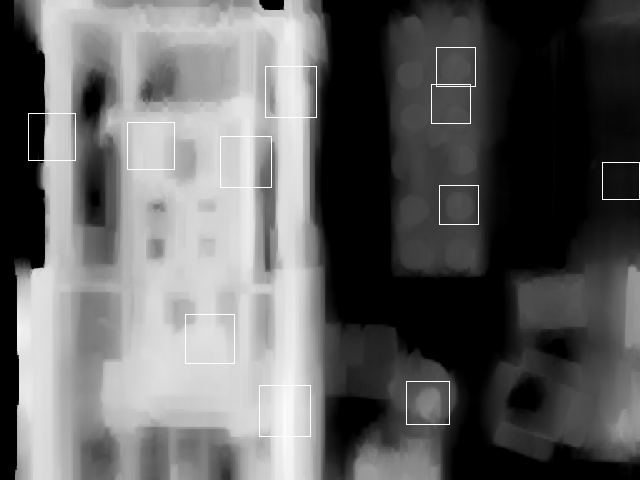
\includegraphics[width=0.45\linewidth]{dataset/0.png}}%

\subfloat[]{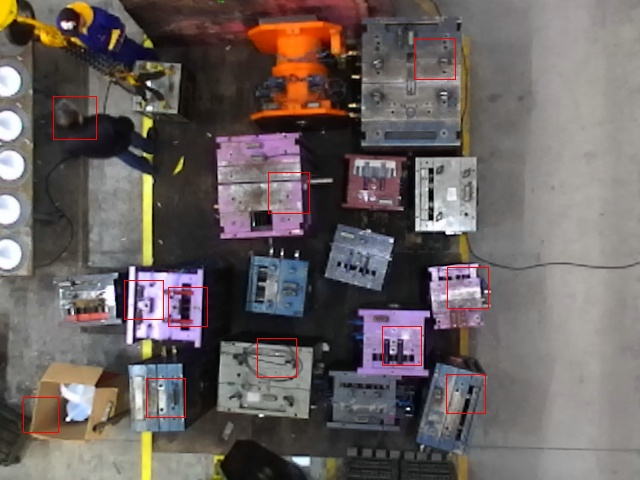
\includegraphics[width=0.45\linewidth]{dataset/19.jpg}}%
\hfil
\subfloat[]{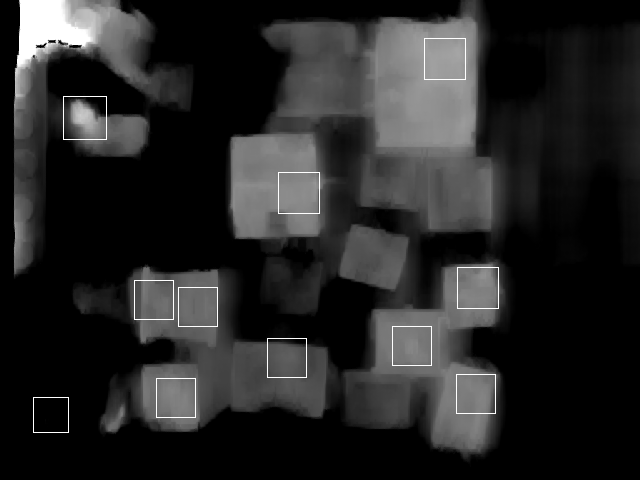
\includegraphics[width=0.45\linewidth]{dataset/19.png}}%

\subfloat[]{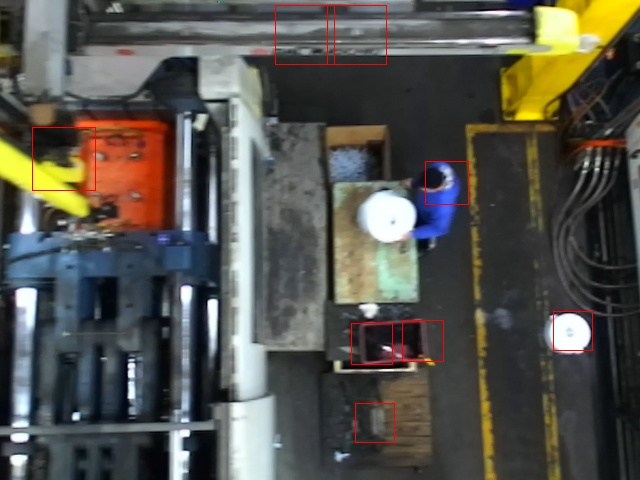
\includegraphics[width=0.45\linewidth]{dataset/20.jpg}}%
\hfil
\subfloat[]{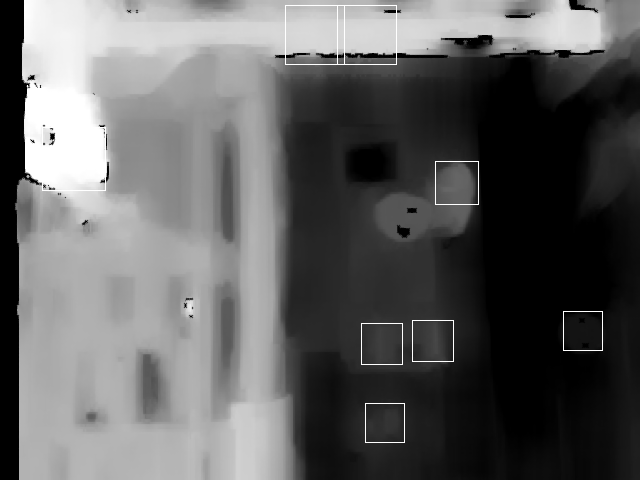
\includegraphics[width=0.45\linewidth]{dataset/20.png}}%
\caption{Dataset examples. Images in first column are RGB and on the right are corresponding depth images. The bounding boxes in the images are obtained by the candidate detection algorithm.}
\label{fig:dataset}
\end{figure*}


\section{Results}
\label{sec:results}

    The evaluation uses Receiver Operating Characteristic (ROC) curves \cite{evaluationMetrics} to compare between descriptors and classifiers. These curves are generated from the probabilistic output of the classifiers used. In the case of SVM which under original formulations is a non-probabilistic classifier, we use a logistic regression formulation \cite{svmProbabilisticOutput} to enable a probabilistic output. The advantage of using such a probabilistic output classifier is the possibility of adjusting the true-positive vs false-positive trade-off even after training, by choosing the probability threshold above which the sample is considered to be positive.

    To evaluate the solutions proposed on Sections \ref{sec:classical} and \ref{sec:deep}, with their variations, we firstly consider the candidate test set, thus evaluating only the descriptor and classifier. Figure \ref{fig:result-classifiers} shows the performance of the classifiers under the test set and a Area Under Curve (AUC) score \cite{evaluationMetrics}. We note that the concentric rings descriptor generalized better when compared to the traditional block grid descriptor. Even then, the deep based classifier outperforms the traditional hand-engineered feature extraction based approach by a large margin.


    \begin{figure*}[!t]
    \centering
    \subfloat[]{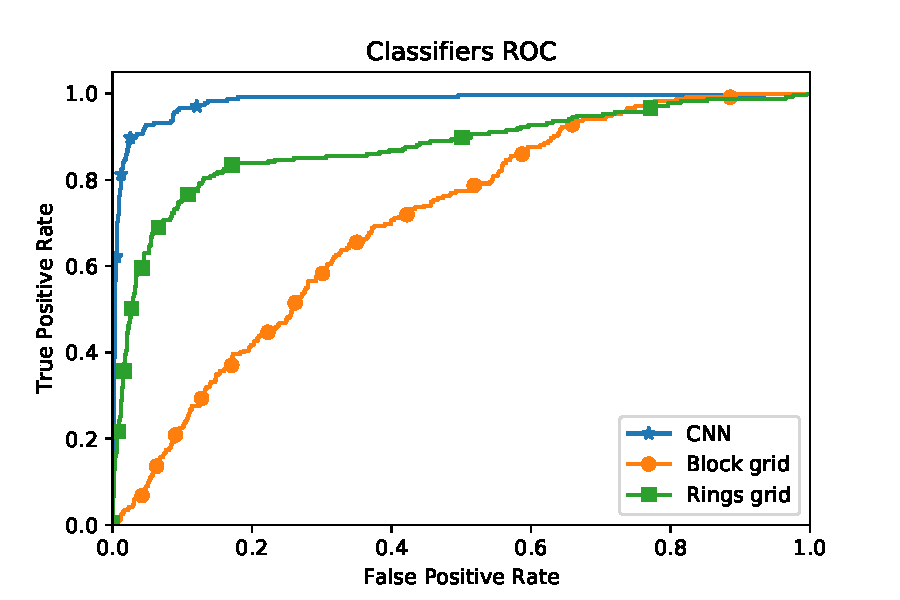
\includegraphics[width=0.45\linewidth]{results/ROC_classifiers.pdf}}%
    \label{fig:result-classifiers-all}
    \hfil
    \subfloat[Zoom in 10\% FPR]{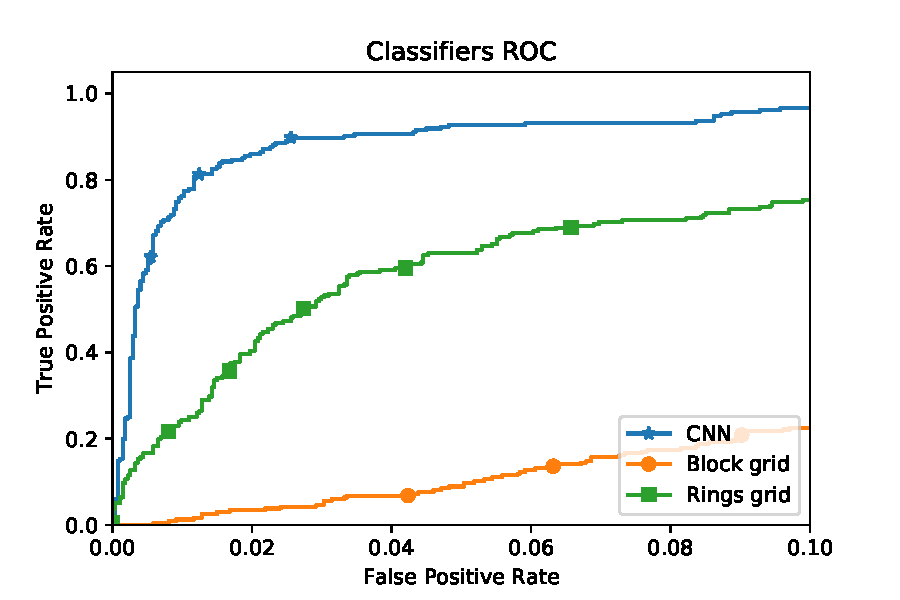
\includegraphics[width=0.45\linewidth]{results/ROC_classifiers_zoom.pdf}}%
    \caption{Classifiers performance. The AUC score for each classifier was, respectively, 0.9810, 0.7019 and 0.8745.}
    \label{fig:result-classifiers}
    \end{figure*}


    In a second phase we consider the overall system performance, including the candidate extraction step. It is important to note that the performance observed in Figure \ref{fig:result-classifiers} is an upper bound of the overall performance, since now there will be miss-detections from the candidate extraction step. Another consideration is that in this phase the we use the whole frame test set, so the probability of the frame contain at least one head could be calculated using
    \begin{equation}
    P[y=1] = 1 - \prod_i^n (1-p_i)
    \end{equation}
    where $y$ is a random variable valued 1 if there are humans in the scene or 0 otherwise, $n$ is the number of candidates and $p_i$ is the classifier output of candidate $i$. Since the CNN classifier offered the best performance we will use this as the final classifier. Figure \ref{fig:result-system} shows the overall system performance using this formulation of the proposed CNN classifier with coarse and fine scales of candidate extraction windows.

    \begin{figure*}[!t]
    \vspace{-3ex}
    \centering
    \subfloat[]{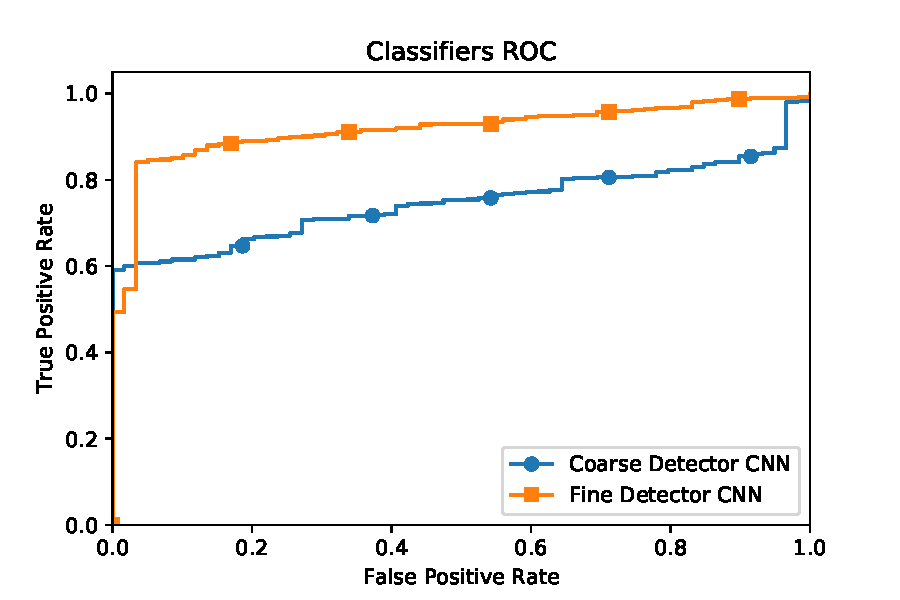
\includegraphics[width=0.45\linewidth]{results/ROC_system.pdf}}
    \label{fig:result-system-all-zoom}
    \subfloat[10 \% interest zone, best results]{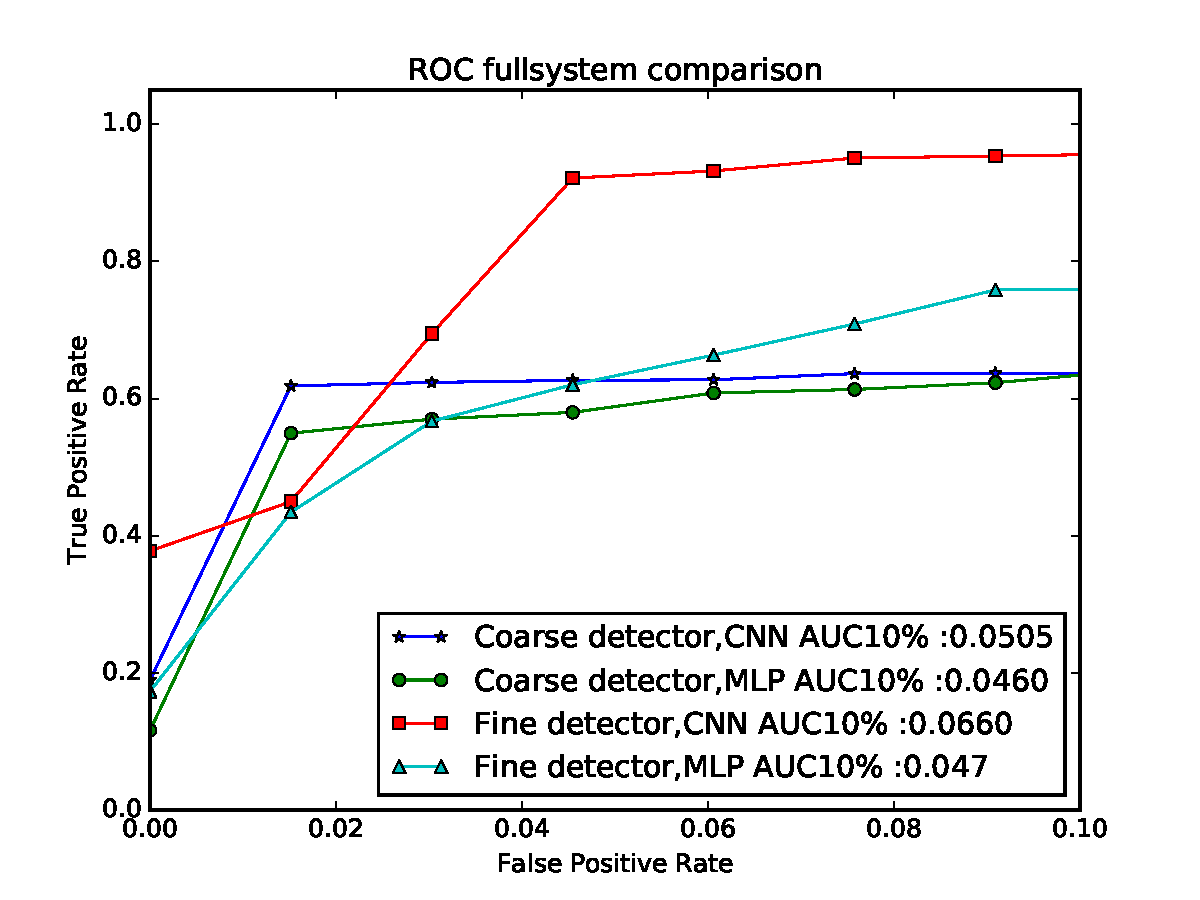
\includegraphics[width=0.45\linewidth]{results/ROC_system_zoom_best.pdf}}%
    \label{fig:result-system}
    \hfil
    \caption{Overall system performance.}
    \end{figure*}


\section{Conclusion}
\label{sec:conclusion}
    This paper investigates two solutions for the human detection problem, one based on traditional computer vision methods and another on deep learning techniques. The results presented in Section \ref{sec:results} show that the last method outperforms traditional hand-engineered feature extraction and classification, although they require a larger training set and have higher complexity, thus requiring more processing power. While deep learning techniques are widely regarded as useful for big datasets, we were still able to achieve good performance, even under a moderate-sized unbalanced dataset.

    One possible direction of future work is investigating a more general CNN structure. Instead of receiving just the candidate window, it would receive the whole depth frame as input and output the probability that frame contains a human. As we saw an improvement of the classification by letting the model choose the best representation of the data, we suspect that allowing the model to access the whole frame as opposed to only small windows possibly containing humans will improve the overall system performance.
